\chapter{Different Approaches for Solving the Drift-Diffusion Equation on Metric Graphs using PINNs}

In this chapter we present different approaches of using a physics informed neural network to solve a set of drift-diffusion equations defined in a given metric graph to given initial and boundary conditions, as described in \cref{ch1:sec2}. These approaches differ in their methodology for training the neural networks used to approximate the solution \cref{Drift-Diffusion-equation} on an individual edge $e \in \mathcal{E}$ under the given conditions. In \cref{ch3:sec1}, we discuss a approach in which the approximation problem on all edges are considered simultaneously in the learning phase. This means that for all edges we combine the deviation of the approximate solution to the drift-diffusion equation and the deviation of the approximate solution to the initial and boundary conditions in one cleverly defined cost function and focus only on solving this single resulting cost function in the learning phase. In \cref{ch3:sec2}, we discuss an approach similar to the idea in \cite{JagtapKharazmiKarniadakis:2020}, where we define a cost function for the approximation problem on each edge of the graph, optimize them one by one, store for each edge certain relevant data for the interconnection of the edges, and repeat this process several times. Thus we have a set of cost functions whose number corresponds to the number of edges, whereby the individual cost functions are minimized several times in succession in the learning phase. The two approaches thus differ in the definition of the cost functions, into which the corresponding neural network and the initial and boundary conditions are incorporated differently, and the sequence in the learning phase, simultaneously or periodically, with which the weights and biases of the corresponding neural network are modified. Furthermore, we use different types and topologies of neural networks for these two approaches in the corresponding sections. We perform numerical experiments for each combination of PINN approach and neural network, and compare the solutions with those generated by the FEM presented in \cref{ch2}. We are particularly interested in the accuracy and efficiency of the different approaches so that we can determine a superior method for solving the approximation problem. In \cref{ch3:sec3}, we compare the performance of a PINN with explicitly calculated derivatives used inside the Hamiltonian, and thus in the corresponding residual network and cost function, with that of a PINN that uses automatic differentiation for this purpose, in order to demonstrate the capabilities of \lstinline!TensorFlow!. \\
In order to compare all the results of all numerical experiments, we use the same problem setup for each experiment, i.e. the set of drift-diffusion equations is considered on the same metric graph $\Gamma$ under the same initial and boundary conditions in each experiment. The metric graph $\Gamma = (\mathcal{V}, \mathcal{E})$ is defined by the following adjacency matrix: 
\begin{equation}
    \label{NumericalExperimentGraph}
    A^{\Gamma} = 
    \begin{blockarray}{ccccccc}
        v_1 & v_2 & v_3 & v_4 & v_5 & v_6 \\
        \begin{block}{(cccccc)c}
            0 & 0 & 1 & 0 & 0 & 0 & v_1 \\
            0 & 0 & 1 & 0 & 0 & 0 & v_2 \\
            0 & 0 & 0 & 1 & 0 & 0 & v_3 \\
            0 & 0 & 0 & 0 & 1 & 1 & v_4 \\
            0 & 0 & 0 & 0 & 0 & 0 & v_5 \\
            0 & 0 & 0 & 0 & 0 & 0 & v_6 \\
        \end{block}
    \end{blockarray}
\end{equation}
The graph $\Gamma$ consists of $6$ vertices $\mathcal{V} = \{ v_i \}_{i = 1,\ldots, 6}$ and $5$ edges $\mathcal{E} = \{ e_i \}_{i = 1,\ldots, 5}$ and is of course directed since $A^{\Gamma}$ is not symmetric. The graph $\Gamma$ is illustrated in \cref{fig7}. 
\begin{figure}[H]
    \begin{center}
        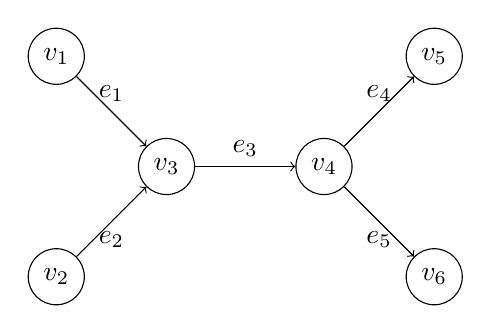
\begin{tikzpicture}
            % vertices
            \node[shape=circle,draw=black] (v1) at (-2.4,1.4) {$v_1$};
            \node[shape=circle,draw=black] (v5) at (2.4,1.4) {$v_5$};
            \node[shape=circle,draw=black] (v3) at (-1,0) {$v_3$};
            \node[shape=circle,draw=black] (v4) at (1,0) {$v_4$};
            \node[shape=circle,draw=black] (v2) at (-2.4,-1.4) {$v_2$};
            \node[shape=circle,draw=black] (v6) at (2.4,-1.4) {$v_6$};
            
            % edges
            \path [->](v1) edge node[above] {$e_1$} (v3);
            \path [->](v2) edge node[below] {$e_2$} (v3);
            \path [->](v3) edge node[above] {$e_3$} (v4);
            \path [->](v4) edge node[above] {$e_4$} (v5);
            \path [->](v4) edge node[below] {$e_5$} (v6);
        \end{tikzpicture}
    \end{center}
    \caption{Will come soon \ldots}
    \label{fig7}
\end{figure}
As we can see, the vertices $v_1$, $v_2$, $v_5$ and $v_6$ are the exterior vertices, i.e. $\mathcal{V}_{\mathcal{D}} = \{v_1, v_2, v_5, v_6\}$, and the vertices $v_3$ and $v_4$ are the interior vertices, i.e. $\mathcal{V}_{\mathcal{K}} = \{v_3, v_4\}$, of the graph $\Gamma$. \\
As an approximation problem, we consider the set of drift-diffusion equations, \cref{Drift-Diffusion-equation}, on all edges $e \in \mathcal{E}$ of the graph $\Gamma = (\mathcal{V}, \mathcal{E})$, defined by \cref{NumericalExperimentGraph}, under the conditions \cref{eq:Kirchhoff_Neumann_condition}, \cref{continuous on vertices}, \cref{eq:Dirichlet_conditions} and \cref{eq:initial_conditions} and under the following assumptions:
\begin{assumption} 
    \ \\[-1.5\baselineskip]
    \begin{enumerate}
        \item The time interval ends at $T = 10$ and the graph $\Gamma$ is equilateral (see \cref{metric graph equilateral}) with $\ell = 1$. 
        \item Let $\varepsilon = 0.01$ in \cref{Drift-Diffusion-equation}.
        \item The mobility in \cref{Drift-Diffusion-equation} is given by $f(\rho_e(t,x)) = \rho_e (t,x)(1-\rho_e (t,x))$.
        \item $\partial_x V_e (t,x) = 1$ for all $(t,x) \in (0, 10) \times [0,1]$ holds in \cref{Drift-Diffusion-equation} for the potential $V_e$ of each edge $e \in \mathcal{E}$. 
        \item On the exterior vertices $\mathcal{V}_{\mathcal{D}}$, we have for flux boundary conditions, \cref{eq:Dirichlet_conditions}, constant influx rates which are specified for $v_1$ by $\alpha_{v_1}(t) = 0.9$ and $\beta_{v_1}(t) = 0$, for $v_2$ by $\alpha_{v_2}(t) = 0.3$ and $\beta_{v_2}(t) = 0$, for $v_5$ by $\alpha_{v_5}(t) = 0$ and $\beta_{v_5}(t) = 0.8$ and for $v_6$ by $\alpha_{v_6}(t) = 0$ and $\beta_{v_6}(t) = 0.1$.
    \end{enumerate}
\end{assumption}
The aim is to compare the performance of the above mentioned two different approaches with different types of neural networks and different topologies of the neural networks. The performance of each approach is determined by its accuracy and its efficiency. To compare the accuracy we use as ground truth the values generated by the finite volume method described in \cref{ch2} with the time discretization $N_t = 5000$ and the space discretization $N_e = 1001$ as a benchmark and measure the difference between them and the values of the trained neural network of the corresponding approach evaluated at the same grid points given by the discretization. In order to compare the efficiency, we measure on the one hand the memory usage needed to create the neural networks and train them, and on the other hand we measure the time needed to execute the implementation of each approach, considering the training and the evaluating of the values at the grid points. \\
The numerical experiments are implemented in \lstinline!Python! 3.8.8 and were run on a Lenovo ThinkPad L490, 64 bit Windows system, 1.8 Ghz Intel Core i7-8565U and 32 GB RAM.
% \lstinline!Jupyter! notebooks 6.3.0 (see \cite{Kluyver:2016}), 
% \lstinline!TensorFlow! 2.5.2.

\section{One Neural Network for all edges}
\label{ch3:sec1}

In this section we construct, in some sense, a global cost function, which is used to train the weights and biases of a neural network by minimizing it in the learning phase, and we perform numerical tests with three different types of neural networks used in this PINN approach. In the following we denote this cost function by $\Phi_\theta$, where $\theta$ only refers to the set of trainable parameters of the used neural network and does not obtain any information about the used type of neural network or the topology of the used neural network. The idea of this approach in this section is that in the learning phase the drift-diffusion equations on all edges and all initial and vertex conditions are considered at once such that all edges are seen as being merged together and thus the problem of approximating the solution of the set of drift-diffusion equations on a metric graph is treated as a whole. Therefore, we construct only one cost function $\Phi_\theta$, which consists of several misfit terms, as in \cref{MSE PINN}, by incorporating the mean-squared-error of a residual network as well as a number of misfit terms which enforce the initial and vertex conditions at a set of collocation points. Of course, we want to exploit the special structure of the domain given by the metric graph for the construction of this cost function $\Phi_\theta$. We note that we set up this cost function $\Phi_\theta$ for the general case and we do not refer for the moment to the values given by the metric graph defined for the numerical experiments by \cref{NumericalExperimentGraph} or by the \cref{graph_assumptions}. \\

We start with the definition of the residual network, which returns the error of the neural network with respect to the fulfillment of \cref{Drift-Diffusion-equation} in the cost function $\Phi_\theta$ at a collocation point. For that, of course, we need a surrogate network, which we denote by $\rho_{\theta_e} \colon \mathbb{R}^2 \to \mathbb{R}$, and which is supposed to approximate the solution $\rho_e$ of \cref{Drift-Diffusion-equation} on an individual edge $e \in \mathcal{E}$. We note that although the surrogate network $\rho_{\theta_e}$ is defined over the entire space $R^2$, it can be assumed that only values from $\left( 0, T \right) \times [0, \ell_e]$ are used, since this is the definition domain of the solution $\rho_e$ to be approximated. Here $\theta_e$ denotes the trainable parameters that are involved in the approximation of $\rho_e$ on an individual edge $e \in \mathcal{E}$, and $\theta_e$ also contains no information about the used type of neural network or the topology of the used neural network. If we insert the surrogate network $\rho_{\theta_e}$ into the right-hand side of \cref{eq:Hamiltonian}, we obtain as a residual network for each individual edge $e \in \mathcal{E}$
\begin{equation}
    \label{Drift-Diffusion residual network}
    r_{\theta_e} \left( t,x \right)=\partial_t \rho_{\theta_e} \left( t,x \right) - \partial_x   \left(  \varepsilon \partial_x  \rho_{\theta_e} \left( t,x \right) - f \left( \rho_{\theta_e} \left( t,x \right) \right) \partial_x V \left( t,x \right) \right).
\end{equation}
Using \cref{Drift-Diffusion residual network} we enforce the structured information imposed by \cref{Drift-Diffusion-equation} for each individual edge $e \in \mathcal{E}$ via
\begin{equation} 
    \label{misfit:residual}
    \phi_{e,r}  \left( X_e \right) \coloneqq \frac{1}{n_e} \sum_{i=1}^{n_e} r_{\theta_e}  \left( x_e^i, t_e^i \right)^2,
\end{equation} 
where $X_e = \{ \left( t_e^i, x_e^i \right)\}_{i=1}^{n_e} \subset \left( 0, T \right) \times [0, \ell_e]$ is a set of time-space collocation points that are drawn randomly or chosen equidistantly. \\
To enforce the Kirchhoff-Neumann conditions, \cref{eq:Kirchhoff_Neumann_condition}, we define the following misfit term for each interior vertex $v \in \mathcal{V}_\mathcal{K}$ 
\begin{equation} 
    \label{misfit:Kirchhoff}
    \phi_{v,K}  \left( X_{v,b} \right) \coloneqq \frac{1}{n_b} \sum_{i=1}^{n_b}  \left( \sum_{e \in \mathcal{E}_v}  \left( - \varepsilon \partial_x \rho_{\theta_e}  \left( t_{v,b}^i, v \right) + f \left( \rho_{\theta_e}  \left( t_{v,b}^i, v \right) \right) \partial_x V_e \left( t_{v,b}^i, v \right) \right) \, n_e  \left( v \right) \right)^2, 
\end{equation} 
where $X_{v,b} = \left\{ t_{v,b}^i \right\}_{i=1}^{n_b} \subset \left( 0,T \right)$ is a set of time snapshots where the Kirchhoff-Neumann conditions are enforced. The values $\left\{ \rho_{\theta_e}  \left( t_{v,b}^i, v \right) \right\}_{i=1}^{n_b}$ are either equal to $\left\{ \rho_{\theta_e}  \left( t_{v,b}^i, 0 \right) \right\}_{i=1}^{n_b}$ if the interior vertex $v \in \mathcal{V}_\mathcal{K}$ is an origin vertex of the edge $e$ (i.e. $\operatorname{o}(e) = v$), or equal to $\left\{ \rho_{\theta_e}  \left( t_{v,b}^i, \ell_e \right) \right\}_{i=1}^{n_b}$ if $v$ is a terminal vertex of the edge $e$ (i.e. $\operatorname{t}(e) = v$). Of course this also applies to the values $\left\{ \partial_x \rho_{\theta_e}  \left( t_{v,b}^i, v \right) \right\}_{i=1}^{n_b}$. We note that the derivatives are taken into the outgoing direction. \\
In order to enforce the continuity in the interior vertices $\mathcal{V}_\mathcal{K}$, required by \cref{continuous on vertices}, we introduce two different misfit terms to accomplish this. In the numerical experiments, we draw attention to which of the two misfit terms is used. The first misfit term is defined for each interior vertex $v \in \mathcal{V}_\mathcal{K}$ by 
\begin{equation} 
    \label{misfit:continuity}
    \phi_{v,c}  \left( X_{v,b} \right) \coloneqq \frac{1}{n_b} \sum_{e \in \mathcal{E}_v} \sum_{i=1}^{n_b} \left(  \rho_{\theta_e}  \left( t_{v,b}^i, v \right) - \rho_{v}^i \right)^2,
\end{equation} 
with $X_{v,b} = \{t_{v,b}^i\}_{i=1}^{n_b}$ as introduced before. Here, we introduce for each interior vertex $v \in \mathcal{V}_\mathcal{K}$ some additional trainable parameters $\left\{ \rho_{v}^i \right\}_{i=1}^{n_b}$, that are appended to $\theta$ and which are also trained by minimizing the resulting cost function $\Phi_\theta$. The other misfit term is defined for each interior vertex $v \in \mathcal{V}_\mathcal{K}$ by 
\begin{equation} 
    \label{misfit:continuity:average}
    \phi_{v,c}  \left( X_{v,b} \right) \coloneqq \frac{1}{n_b}  \sum_{i=1}^{n_b} \left( \sum_{e \in \mathcal{E}_v} \left( \rho_{\theta_e}  \left( t_{v,b}^i, v \right) - \frac{1}{\abs{\mathcal{E}_v}} \sum_{e \in \mathcal{E}_v} \rho_{\theta_e}  \left( t_{v,b}^i, v \right) \right) \right)^2.
\end{equation}
Here, on average over all time collocation points $\left\{ t_{v,b}^i \right\}_{i=1}^{n_b}$, the value $\rho_{\theta_e}  \left( t_{v,b}^i, v \right)$ of each edge $e \in \mathcal{E}_v$ should be equal to the average of all edges connected to this interior vertex $v \in \mathcal{V}_\mathcal{K}$. Both misfit terms have their numerical advantages and disadvantages. The misfit term defined by \cref{misfit:continuity} is not so complex, from which can follow that the derivatives with respect to the trainable parameters $\theta$ in the used optimization method is easier to compute, but therefore adds \cref{misfit:continuity} just as much trainable parameters as collocation points to the set of trainable parameters. No further trainable parameters need to be added for the misfit term given by \cref{misfit:continuity:average}, but it is more complex for that. \\
We enforce the flux vertex conditions given by \cref{eq:Dirichlet_conditions} for each exterior vertex $v \in \mathcal{V}_\mathcal{D}$ by defining the following misfit term  
\begin{align} 
    \label{misfit:Dirichlet}
    \phi_{v,D}  \left( X_{v,b} \right) \coloneqq & \frac{1}{n_b} \sum_{i=1}^{n_b} \bigg( \sum_{e \in \mathcal{E}_v} \left(- \varepsilon \partial_x \rho_{\theta_e}  \left( t_{v,b}^i, v \right) + f\left(\rho_{\theta_e}  \left( t_{v,b}^i, v \right)\right) \partial_x V_e\left( t_{v,b}^i, v \right) \right) n_e  \left( v \right) + \\
    & \alpha_v \left( t_{v,b}^i \right)  \left( 1- \rho_{\theta_e}  \left( t_{v,b}^i, v \right) \right) - \beta_v \left( t_{v,b}^i \right) \rho_{\theta_e}  \left( t_{v,b}^i, v \right) \bigg)^2
\end{align}
with $X_{v,b} = \{t_{v,b}^i\}_{i=1}^{n_b}$ as introduced before. \\
To enforce the initial conditions for each edge $e \in \mathcal{E}$, \cref{eq:initial_conditions}, we define the following misfit term  
\begin{equation} 
    \label{misfit:initial}
    \phi_{e,0}  \left( X_{e,0} \right) \coloneqq \frac{1}{n_0} \sum_{i=1}^{n_0}  \left( \rho_{\theta_e}  \left( 0,x_{e,0}^i \right) - \rho_{e,0} \left( x_{e,0}^i \right) \right)^2, 
\end{equation} 
where $X_{e,0} = \{x_{e,0}^i\}_{i=1}^{n_0} \subset [0, \ell_e]$ is a set of collocation points along $t=0$. \\ 
Now we combine all misfit terms defined above to form the cost function $\Phi_\theta$ by adding the different mean values over the units in which the concerned misfit term is applicable: 
\begin{align} 
    \label{eq:loss:1}
    \Phi_{\theta} \left( X_{data} \right) & =  \frac{1}{\abs{\mathcal{V}_\mathcal{D}}} \sum_{v \in \mathcal{V}_\mathcal{D}} \phi_{v,D} \left( X_{v,b} \right) + \frac{1}{\abs{\mathcal{V}_\mathcal{K}}} \sum_{v \in \mathcal{V}_\mathcal{K}}  \left(  \phi_{v,K}  \left( X_{v,b} \right) + \phi_{v,c} \left( X_{v,b} \right)  \right) + \\
    & \quad + \frac{1}{\abs{\mathcal{E}}} \sum_{e \in \mathcal{E}}  \left(  \phi_{e,r}  \left( X_{e,r} \right) + \phi_{e,0}  \left( X_{e,0} \right)  \right), 
\end{align}
where $X_{data}$ represents the union of the different collocation points $X_e$, $X_{v,b}$ and $X_{e,0}$. In the learning phase, this cost function $\Phi_{\theta}$ is minimized with respect to the trainable parameters $\theta$, in the hope that the resulting trained surrogate network $\rho_{\theta_e}$ for each edge $e \in \mathcal{E}$ will approximate the solution of the drift diffusion equation given by \cref{Drift-Diffusion-equation} well to a certain degree under the given initial and vertex conditions. 

So far we have not specified what type of neural network with which topology we use for $\rho_{\theta_e}$, i.e. to approximate the solution of \cref{Drift-Diffusion-equation} on an individual edge $e \in \mathcal{E}$ under the given initial and vertex conditions. Of course, we have an infinite freedom of choice, the only constraints being the dimension of the input $(x,t) \in \mathbb{R}^2$, the dimension of the output $\rho_{\theta_e}(t, x) \in \mathbb{R}$ and the differentiability of the corresponding neural network up to order two (due to $\partial_{xx} \rho_{\theta_e}$ appears in \cref{Drift-Diffusion-equation}). We now introduce three different types of neural network for the approximation of $\rho_e \colon (0, T) \times [0, \ell_e] \to \mathbb{R}$, which we use in the numerical experiments. \\
Since we have to find an approximation $\rho_{\theta_e}$ for each edge $e \in \mathcal{E}$ and since these approximations $\left\{ \rho_{\theta_e} \right\}_{e \in \mathcal{E}}$ are individually included in the cost function $\Phi_{\theta}$, it is quite evident to use one single neural network for the approximation of the solution of \cref{Drift-Diffusion-equation} on one individual edge $e$. This results in the fact that we use as many neural networks as we have edges of the graph $\Gamma$. In this case, $\theta_e$ describes the trainable parameters of a single neural network and $\theta$ is the union of the trainable parameters of all neural networks. Thus, during the learning phase, all trainable parameters $\theta$ are modified when the cost function $\Phi_{\theta}$ is minimized, and therefore consider the used optimization methods $\theta$ as the optimization variable. Using one neural network for the approximation of the solution on one edge offers the possibility to select individual hyperparameters like the topology or the activation functions for the different neural networks. One can use a deep neural network for an edge for which the solution can have a complex structure, while a shallow neural network can be used on the edges with relatively simple and smooth solutions. In this work, however, we will not cover such a case due to the effort of finding the best hyperparameters for each neural network, we just use the same type of neural network with the same topology for the approximation of $\rho_e$ each edge $e \in \mathcal{E}$. \\

% Noch die richtigen Hyperparameter hinzufügen
We adopt this approach of using a single neural network to approximate $\rho_e$ on a single edge $e \in \mathcal{E}$ for the numerical experiments and we use two different types of neural networks for that. For the first numerical experiment, we use for $\rho_{\theta_e}$ a feed-forward neural network, denoted by $fnn_{\theta_e}$, with $L$-layers for each edge $e \in \mathcal{E}$, which is defined by 
\begin{gather}
    \label{one_for_each}
    fnn_{\theta_e} \colon \mathbb{R}^2 \to \mathbb{R}, \\
    \\
    fnn_{\theta_e}(x, t) = \sigma_L(W^L \sigma_{L-1}(W^{L-1}\sigma_{L-2}(\cdots \sigma_{1}(W^{1}x^0 +b^1) \cdots) + b^{L-1}) + b^{L}),
\end{gather}
where $x^0 = (t, x)^{\mathrm{T}} \in (0, T) \times [0, \ell_e] \subset \mathbb{R}^2$ and $\theta_e = \left\{ \left\{ W^l \right\}_{l = 1, \ldots, L}, \left\{ b^l \right\}_{l = 1, \ldots, L} \right\}$ with $W^l \in \mathbb{R}^{n_l \times n_{l-1}}$ and $b^l \in \mathbb{R}^{n_l}$, where $n_0 = 2$ and $n_L = 1$. The total set of all trainable parameters for the resulting PINN approach is therefore $\theta = \bigcup_{e \in \mathcal{E}} \ \theta_e$. Feed-forward neural networks have already been used in various PINN setups, so this choice can be considered as reasonable.  \\
For the second numerical experiment, we use for $\rho_{\theta_e}$ a neural network, which is defined by the following architecture and the following forward propagation
\begin{gather}
    \label{Resnet1}
    R_{\theta_e} \colon \mathbb{R}^2 \to \mathbb{R}, \\
    \\
    R_{\theta_e}(t,x) = \frac{1}{2} {x^0}^{\mathrm{T}} A x^0 + w^{\mathrm{T}} x^{L} + c^{\mathrm{T}} x^0,
\end{gather}
with
\begin{gather}
    \label{Resnet2}
    x^1 = \sigma_1(W^1 x^{0} + b^1) \in \mathbb{R}^m, \\
    \\
    x^l = x^{l-1} + h \cdot \sigma_l(W^l x^{l-1} + b^l) \in \mathbb{R}^m \quad \text{for} \quad l = 2, \ldots, L, 
\end{gather}
where $h > 0$ is called stepsize and is a hyperparameter, $x^0 = (t, x)^{\mathrm{T}} \in (0, T) \times [0, \ell_e] \subset \mathbb{R}^2$, $W^1 \in \mathbb{R}^{m \times 2}$ and $W^l \in \mathbb{R}^{m \times m}$ for $l = 2, \ldots, L$, $b^l \in \mathbb{R}^{m}$ for $l = 1, \ldots, L$ and $A \in \mathbb{R}^{2 \times 2}$, $w \in \mathbb{R}^m$, $c \in \mathbb{R}^2$ are also trainable parameters, i.e. $\theta_e = \left\{ \left\{ W^l \right\}_{l = 1, \ldots, L}, \left\{ b^l \right\}_{l = 1, \ldots, L}, A, w, c \right\}$ and $\theta = \bigcup_{e \in \mathcal{E}} \ \theta_e$. The idea of using this type of neural network originates from \cite{RuthottoOsherLiNurbekyanFung2020}, in which high-dimensional mean field games and mean field control models are approximately solved by combining Lagrangian and Eulerian viewpoints and by using a tailored neural network parameterization for the potential of the solution, which can be understood as a density, to avoid any spatial discretisation. The neural network given by the forward propagation in \cref{Resnet2} is also called residual network and abbreviated with ResNet, \cite{HeZhangRenSun:2015}. We refer to it only as ResNet to avoid confusion with the residual network of a PINN. ResNets have been successful in a wide range of machine learning tasks and have been found to be trainable even for many layers. By interpreting \cref{Resnet2} as a forward Euler discretization of an initial value problem, the continuous limit of a ResNet is amenable to mathematical analysis, \cite[p.~6]{RuthottoOsherLiNurbekyanFung2020}. \\

For a further numerical experiment we use a completely different approach of utilizing a neural network to approximate the solutions of the set of drift-diffusion equations. We use one single feed-forward neural network with $L \in \mathbb{N}$ layers for the approximation of the solution of \cref{Drift-Diffusion-equation} under the given initial and vertex conditions on all edges of the graph $\Gamma$, i.e. this network returns for a point $(t,x) \in \mathcal{R}^2$ the values $\rho_{\theta_{e_i}}(x, t)$ for all edges $\mathcal{E} = \left\{ e_i \right\}_{i = 1, \ldots, E}$, where $E = \abs{\mathcal{E}}$. We define this neural network as follows
\begin{gather}
    \label{one_for_all}
    \mathfrak{FNN}_{\theta} \colon \mathbb{R}^2 \to \mathbb{R}^E \\
    \\
    \mathfrak{FNN}_{\theta}(x, t) = \sigma_L(W^L \sigma_{L-1}(W^{L-1}\sigma_{L-2}(\cdots \sigma_{1}(W^{1}x^0 +b^1) \cdots) + b^{L-1}) + b^{L}) \in \mathbb{R}^E, 
\end{gather}
where $x^0 = (t, x)^{\mathrm{T}} \in (0, T) \times [0, \ell_e] \subset \mathbb{R}^2$ and $\theta = \left\{ \left\{ W^l \right\}_{l = 1, \ldots, L}, \left\{ b^l \right\}_{l = 1, \ldots, L} \right\}$ with $W^l \in \mathbb{R}^{n_l \times n_{l-1}}$ and $b^l \in \mathbb{R}^{n_l}$, where $n_0 = 2$ and $n_L = E$. The individual approximations are given by 
\begin{equation*}
    \rho_{\theta_{e_i}}(x, t) = \left[ \mathfrak{FNN}_{\theta}(x, t) \right]_i \in \mathbb{R},
\end{equation*}
i.e. the $i$-th entry of the networks output $\mathfrak{FNN}_{\theta}(x, t) \in \mathbb{R}^E$ is the approximation of the solution on the $i$-th edge. We see that in this case $\theta$ consists only of the weights and biases of this single network, as indicated by the index $\theta$ in $\mathfrak{FNN}_{\theta}$. \\
The use of a single neural network is motivated by the hope that the neurons in the hidden layers will learn the structure of the entire graph and the resulting communication of the edges via the vertices, i.e. that all interactions within the graph are taken into account by the neurons after the learning phase. Furthermore, we hope that the computational cost is reduced, since only the weights and biases of this single network need to be trained, provided the depth and width of the neural network $\mathfrak{FNN}_{\theta}$ are not too large. The fact that $\mathfrak{FNN}_{\theta}(x, t)$ generates the output for all edges at the same time is also an advantage, as in an implementation only the execution of one network is necessary instead of several. However, we point out that this approach only makes sense if the graph is equilateral, see \cref{graph_assumptions}, because then the same collocation points $X_e = \{ \left( t_e^i, x_e^i \right)\}_{i=1}^{n_e}$ and $X_{e,0} = \{x_{e,0}^i\}_{i=1}^{n_0}$ can be used for the misfit terms given by \cref{misfit:residual} and \cref{misfit:initial} for all edges $e \in \mathcal{E}$. 


With the cost function defined by \cref{eq:loss:1} and the three different types of neural networks defined above, we perform numerical experiments in which these neural networks are trained by this cost function for the approximation problem, which is given by the set of drift-diffusion equations given by \cref{Drift-Diffusion-equation} on the metric graph defined by \cref{NumericalExperimentGraph} under the initial and vertex conditions and the given \cref{graph_assumptions}. The time required for the learning phase is measured and then the deviation of the values generated by these neural networks at the grid points from the values generated by the FVM at these grid points is measured. \\
As mentioned before, these are implemented in \lstinline!Python 3.8.8!. All collocation points listed after that are randomly generated using \lstinline!tf.random.uniform!, which is provided by the package \lstinline!Tensorflow! and uses an normal distribution. Further we set \lstinline!dtype = 'float64'!. As time-space collocation points $X_e$ for \cref{misfit:residual} we use $n_e = 4000$ randomly selected points $\left\{ \left( t_e^i, x_e^i \right) \right\}_{i=1}^{n_e} \subset \left( 0, T \right) \times [0, \ell_e]$. As space collocation points $X_{e,0}$ for \cref{misfit:initial} we use $n_0 = 1000$ randomly selected points $ \left\{ x_{e,0}^i \right\}_{i=1}^{n_0} \subset [0, \ell_e]$. For \cref{misfit:Kirchhoff}, \cref{misfit:Dirichlet}, \cref{misfit:continuity} or \cref{misfit:continuity:average} we use $n_b = 1000$ randomly chosen points $\left\{ t_{0,b}^i \right\}_{i=1}^{n_b} \subset \left( 0,T \right)$ as time snapshots $X_{0,b}$ for origin vertices, i.e. $v = 0$, and $n_b = 1000$ randomly chosen points as time snapshots $X_{\ell,b}$ for terminal vertices, i.e. $v = 0$ (we recall that the graph $\Gamma$ is equilateral).











% Kollokationspunkte 

We note that, as mentioned in \cref{ch1:sec4}, all derivatives of surrogate models with respect to the input parameters are computed with automatic differentiation provided by \lstinline!Tensorflow! via the method \lstinline!tf.GradientTape!. We use 


For the minimization of the cost function $\Phi_{\theta}$, we first use a variant of the gradient descent method, in which the direction is given by the Adam optimizer from the module \lstinline!Keras!, see \cite{Chollet:2015}, which belongs to the package \lstinline!Tensorflow!, see \cite{TensorFlow}. We change for the different types of neural networks the input parameter \lstinline!learning_rate!, which obviously specifies the learning rate of the method, and leave all other input parameters of the Adam optimizer by default. This method stops after 2000 iterations. After that, we use the L-BFGS-B optimizer from the package \lstinline!SciPy!, see \cite{SciPy:2020}, and we set for all networks as parameters in the options \lstinline!maxiter = 5000! which specifies the maximum number of iterations, \lstinline!maxfun = 50000! which specifies the maximum number of function evaluations, \lstinline!maxcor = 50! which specifies the maximum number of stored variable metric corrections used in the L-BFGS approximation of the Hessian of the cost function $\Phi_{\theta}$, \lstinline!maxls = 50! which specifies the maximum number of line search steps per iteration and \lstinline!ftol = 1.0*np.finfo(float).eps! which specifies a parameter in a stopping criterion that aborts the method if the values of the cost function $\Phi_{\theta}$ between two iterates are too small.


\begin{table}[H]\label{tab:one_cost_function}
    \resizebox{\textwidth}{!}{
        \begin{tabular}{l l l l }
            \toprule
            Neural Network given by & One each egde & Resnet & One  \\ 
            \midrule
            Error & $0.15$ & $0.21$ & $0.54$ \\ 
            \midrule
            Time in seconds & $0.15$ & $0.21$ & $0.54$  \\ 
            \midrule
            Number of Iterations & $72$ & $68$ & $72$ \\
            \bottomrule
        \end{tabular}
    }
    \caption{Comparison of different types of neural networks.}
\end{table}
\section{One Neural Network for each edge}
\label{ch3:sec2}

In this section, we present a PINN approach for solving the set of drift-diffusion equations on a metric graph, where a cost function for the approximation of $\rho_e \colon (0,T) \times [0, \ell_e] \to [0, 1]$ is defined for each edge $e \in \mathcal{E}$ of the graph $\Gamma = (\mathcal{V}, \mathcal{E})$, where the included misfit terms are defined in such a way that the solution of the approximation problem on the entire graph is ensured. The idea for this approach is adopted from \cite{JagtapKharazmiKarniadakis:2020}, in which so-called conservative physics-informed neural networks, abbreviated cPINNs, on discrete domains for non-linear conservation laws were presented. In \cite{JagtapKharazmiKarniadakis:2020} the domain on which the relevant conservation law is defined is split into several adjacent subdomains and one neural network is used as a PINN to solve the conservation law in one subdomain. The conservation property is achieved on the whole domain by enforcing the flux continuity in the strong form along the intersections of these subdomains. Apart from the flux continuity condition, an average solution given by two different neural networks is also enforced at the common interface between two sub-domains. The cost function of cPINN is defined for each subdomain, which has a similar structure as the PINN cost function in each subdomain, but these two interface conditions are incorporated by misfit terms. Consequently, one has as many cost functions as subdomains into which one has split the original domain. These cPINN cost functions are then minimized several times in succession with an optimization method, such as SGD, with respect to their learnable parameters dependent on the corresponding subdomain, and certain values, which are needed e.g. for the average solution at the common interface between two sub-domains, are stored. The splitting into several subdomains allows to use neural networks with different architectures for each subdomain to obtain the solution of the same underlying PDE, and also allows to choose different non-learnable hyperparameters such as the type of optimization method for the minimization in the learning phase. Also there is a possibility to train the networks in parallel, i.e., simultaneously, which is very important in terms of achieving computational efficiency. The domain decomposition in the cPINN approach together with the use of an individual neural network for the different subdomains offers as an advantage the possibility for the reduction of the approximation error. \\
We adopt for our approach this idea of splitting the domain into several subdomains and receiving an individual cost function for each subdomain. For this purpose, we associate the individual subdomains with the individual edges of the considered graph, i.e. we construct now a cost function for each edge of the considered graph. These cost functions for all edges are minimized several times in succession, always training only the learnable parameters that are needed to approximate the solution on exactly this edge.\\
We now construct the cost function for the approximation of the solution of \cref{Drift-Diffusion-equation} on a single edge, which we denote by $\hat{e} \in \mathcal{E}$ to distinguish it more easily from the other edges $e \in \mathcal{E} \setminus \{ \hat{e}\}$. In the following, we denote the cost function for an individual edge by $\Phi_{\theta_{\hat{e}}}$, where $\theta_{\hat{e}}$ denotes the learnable parameters which are used for the approximation of $\rho_{\hat{e}}$. Like the cost functions given by \cref{eq:loss:1} and \cref{MSE PINN}, the cost function $\Phi_{\theta_{\hat{e}}}$ consists also of several misfit terms. \\
Since we require that the corresponding neural network approximates the solution of the drift-diffusion equation on the edge e, therefore we incorporate the mean squared error of the residual network given by \cref{Drift-Diffusion residual network}

the term given by Equation 3 into our cost function.  

Two misfit terms always appear the same, term 1 and term 2, where we can simply incorporate equation 1 and equation 2 into the cost function here. 

Each edge is defined by two vertices which it connects and by which it is linked to other edges. When we construct a cost function for an individual edge, both vertices must be checked to see if they are either an interior or an exterior vertex, since it follows that different conditions apply and thus different terms are incorporated into the cost function. 

Fortunately, we can incorporate two terms from Section 2, the term for the residual network and the term for the initial condition. This is because these terms are defined for each edge individually and the average of these terms over all edges is incorporated in the final cost function. Here we do not incorporate the average of all edges into the cost function, but only the term for one edge. This is to ensure that the trained neural network approximates the solution of the equation on this edge and satisfies the initial conditions.  \\

What the interface conditions are in \cite{JagtapKharazmiKarniadakis:2020} are here the vertex conditions that couple the edges at a vertex, i.e., \cref{eq:Kirchhoff_Neumann_condition} and \cref{continuous on vertices} on the interior vertices $\mathcal{V}_\mathcal{K}$ and \cref{eq:Dirichlet_conditions} on the exterior vertices $\mathcal{V}_\mathcal{D}$. 

Each edge is defined by two vertices which it connects and by which it is linked to other edges. When we construct a cost function for an individual edge, both vertices must be checked to see if they are either an interior or an exterior vertex, since it follows that different conditions apply and thus different terms are incorporated into the cost function. 

To enforce the Kirchhoff-Neumann condition on an interior vertex $v \in \mathcal{V}_\mathcal{K}$, \cref{eq:Kirchhoff_Neumann_condition}, we use the misfit term given by \cref{misfit:Kirchhoff}, but we rewrite it, so that it is apparent that only the learnable parameters, which are necessary for the approximation of the solution on the corresponding edge, are trained. The misfit term for an interior vertex $v \in \mathcal{V}_\mathcal{K}$ is given by
\begin{equation} 
    \label{misfit:Kirchhoff.}
    \phi_{v,K}  \left( X_{v,b} \right) \coloneqq \frac{1}{n_b} \sum_{i=1}^{n_b}  \left( \sum_{e\in \mathcal{E}_v} J_e(t,v) n_e (v) \right)^2, 
\end{equation} 
where $X_{v,b} = \{t_{v,b}^i\}_{i=1}^{n_b} \subset \left( 0,T \right)$ is a set of time snapshots where the Kirchhoff-Neumann conditions are enforced. We note that the derivative is taken into the outgoing direction. \\

When a cost function is trained for one edge, in the optimization procedure the learnable parameters of the networks of the other edges are fixed



If we set up a cost function for an individual edge, then we have to check what these vertices are, because consequently different conditions apply and are included in the cost function. 
\begin{equation}
    \label{vertex funcions}
    \phi_{v}(X_{v,b}) = \begin{cases} \phi_{v,K}  \left( X_{v,b} \right) +  \phi_{v,c}  \left( X_{v,b} \right)& \text{if } v \in \mathcal{V}_{\mathcal{K}}, \\ \phi_{v,D}  \left( X_{v,b} \right) & \text{if } v \in \mathcal{V}_{\mathcal{D}}, \end{cases}
\end{equation}


We define for each edge the cost function $e = (v^{o}_e, v^{t}_e) \in \mathcal{E}$
\begin{equation}
    \label{eq:cost:2}
    \phi_{\theta_e} \left( X_{data} \right) \coloneqq \phi_{e,r}  \left( X_e \right) + \phi_{e,0}  \left( X_{e,0} \right) + \phi_{v^{o}_e}(X_{v,b}) + \phi_{v^{t}_e}(X_{v,b})
\end{equation}
\section{Automatic differentiation vs explicit derivatives}
\label{ch3:sec3}

In this section we show how the neural networks used in the previous numerical tests can be explicitly differentiated so that the use of automatic differentiation in a PINN approach can be omitted. We compare the time to convergence and the computational resources required for a PINN approach programmed in Python with explicit derivatives with the results previously obtained for a PINN that uses automatic differentiation. This aims to show whether an explicit computation of the derivatives for our approximation problem brings computational advantages with it and whether the performance of a PINN approach can be improved as a result. \\
We first consider the case of explicit derivatives with respect to the input of a feed-forward neural network. In this thesis we used two $FNN$s with different topologies, one $FNN$ for each edge of the graph given by \cref{one_for_each} and one $FNN$ for all edges of the graph given by \cref{one_for_all}. We therefore describe the first and second order explicit derivatives of a general $FNN$ and then we will discuss the $FNN$s used in this work. \\
Let this general $FNN$ with $L$ layers be defined by 
\begin{gather}
    \label{model prediction}
    f_{\theta} \colon \mathbb{R}^{n_0} \to \mathbb{R}^{n_L}, \\
    \\
    f_{\theta}\left(x^0\right) = x^L = \sigma_L\left(W^L \sigma_{L-1}\left(W^{L-1}\sigma_{L-2}\left(\cdots \sigma_{1}\left(W^{1}x^0 + b^1\right) \cdots\right) + b^{L-1}\right) + b^{L}\right) \in \mathbb{R}^{n_L}, \\
    \\
    x^l = \sigma_l\left(W^l x^{l-1} + b^l\right) \in \mathbb{R}^{n_l} \quad \text{for} \quad l = 1, \ldots, L,
\end{gather}
where $x^0 \in \mathbb{R}^{n_0}$ and $\theta = \left\{ \left\{ W^L \right\}_{l = 1, \ldots, L}, \left\{ b^L \right\}_{l = 1, \ldots, L} \right\}$ with $W^l \in \mathbb{R}^{n_l \times n_{l-1}}$ and $b^l \in \mathbb{R}^{n_l}$ are the trainable parameters of this network. \\
The first order derivative of this vector-valued map $f_{\theta}\left(x^0\right) \in \mathbb{R}^{n_L}$ with respect to its input $x^0 \in \mathbb{R}^{n_0}$ is a linear map $\frac{\textup{d}}{\textup{d} \ x^0} f_{\theta}\left(x^0\right) \colon \mathbb{R}^{n_0} \to \mathbb{R}^{n_L}$, which can be represented by the Jacobian matrix
\begin{equation}
    \label{Jacobi}
    \frac{\textup{d}}{\textup{d} \ x^0} f_{\theta}\left(x^0\right) = \mathrm{J} \left[f_{\theta} \right]\left(x^0\right) = \begin{pmatrix} \nabla {\left[f_{\theta}\left(x^0\right)\right]_{1}}^{\mathrm{T}} \\ \vdots \\  \nabla {\left[f_{\theta}\left(x^0\right)\right]_{n_L}}^{\mathrm{T}} \end{pmatrix} = \begin{pmatrix} \frac{\partial \left[f_{\theta}\left(x^0\right)\right]_1}{\partial x^0_{1}} & \cdots & \frac{\partial \left[f_{\theta}\left(x^0\right)\right]_1}{\partial x^0_{n_0}} \\ \vdots & \ddots & \vdots \\ \frac{\partial \left[f_{\theta}\left(x^0\right)\right]_{n_L}}{\partial x^0_{1}} & \cdots & \frac{\partial \left[f_{\theta}\left(x^0\right)\right]_{n_L}}{\partial x^0_{n_0}} \end{pmatrix} \in \mathbb{R}^{n_L \times n_0}, 
\end{equation}
where $\left[f_{\theta}\left(x^0\right)\right]_i$ is the $i$-th component of the output $f_{\theta}\left(x^0\right) \in \mathbb{R}^{n_L}$ and $\nabla {\left[f_{\theta}\left(x^0\right)\right]_i}^{\mathrm{T}}$ is the transpose of the gradient of $\left[f_{\theta}\left(x^0\right)\right]_i$. \\
We are interested in deriving the Jacobi matrix for the $FNN$ given by \cref{model prediction}. Since a $FNN$ consists of the composition of (generally) several layers, and each layer consists of the composition of a linear map, which is the propagation function defined in \cref{propagation function}, and a non-linear map, which is activation function defined in \cref{activation function}, we have to apply the chain rule layer by layer, a total of $2L$ many times. We remind that the activation function $\sigma_{l} \colon \mathbb{R}^{n_l} \to \mathbb{R}^{n_l}$ of layer $l$ is defined component-wise, i.e. for $\sigma_{l}\left(a^l\right) \in \mathbb{R}^{n_l}$ holds $\sigma_{l}\left(a^l_i\right) = \left[ \sigma_{l}\left(a^l\right) \right]_i$. Therefore is the Jacobian matrix of the vector-valued activation function $\sigma_{l}\left(a^l\right) \in \mathbb{R}^{n_l}$ of layer $l$ with respect to the activation $a^l = a^l\left(x^{l-1}\right) = W^{l} x^{l-1} + b^{l} \in \mathbb{R}^{n_l}$ of layer $l$ a diagonal matrix, which is defined by
\begin{equation}
    \label{derivative:activation:function}
    \frac{\textup{d}}{\textup{d} \ a^{l}} \ \sigma_{l} \left(a^l\right) = D^{l} = \begin{pmatrix} {\sigma_{l}}^{\prime} \left( a^{l}_1 \right) & & \\ & \ddots & \\ & & {\sigma_{l}}^{\prime} \left( a^{l}_{n_l} \right) \end{pmatrix} \in \mathbb{R}^{n_l \times n_l}, 
\end{equation}
where ${\sigma_{l}}^{\prime} \left( a^{l}_{n_l} \right)$ is the first derivative of the one-dimensional activation function $\sigma_{l} \colon \mathbb{R} \to \mathbb{R}$ applied to the i-th component of $a_l \in \mathbb{R}^{n_l}$. \\
Due to the linearity of the propagation function $a^l = a^l\left(x^{l-1}\right) = W^{l} x^{l-1} + b^{l} \in \mathbb{R}^{n_l}$, its derivative with respect to $x^{l-1} \in \mathbb{R}^{n_{l-1}}$ is simply
\begin{equation}
    \label{derivative:activation}
    \frac{\textup{d}}{\textup{d} \ x^{l-1}} \ a^{l}\left(x^{l-1}\right) = W^l.
\end{equation}
Using equation \cref{derivative:activation:function} and equation \cref{derivative:activation}, we can now differentiate the $FNN$ defined by \cref{model prediction} with respect to its input $x^0 \in \mathbb{R}^{n_0}$ layer by layer to get the Jacobian matrix of \cref{model prediction}
\begin{align}
    \label{first order derivative}
    \frac{\textup{d}}{\textup{d} \ x^0} f_{\theta}\left(x^0\right) & = \frac{\textup{d}}{\textup{d} \ a^{L}} \ \sigma_{L} \left(a^{L}\left(x^{L-1}\right)\right) = \\
    & = D^L \cdot \frac{\textup{d}}{\textup{d} \ x^{L-1}} \ a^{L}\left(x^{L-1}\right) = D^L \cdot \frac{\textup{d}}{\textup{d} \ x^{L-1}} \ \left(W^{L} x^{L-1} + b^{L}\right) = \\
    & = D^L \cdot W^L \cdot \frac{\textup{d}}{\textup{d} \ a^{L_1}} \ \sigma_{L-1} \left(a^{L-1}\left(x^{L-2}\right)\right) = \\
    & = \ldots = \\
    & = D^L \cdot W^L \cdot D^{L-1} \cdot \ldots \cdot W^2 \cdot D^1 \cdot \frac{\textup{d}}{\textup{d} \ x^{0}} \ \left(W^{1} x^{0} + b^{1}\right) = \\
    & = D^L \cdot W^L \cdot D^{L-1} \cdot \ldots \cdot W^2 \cdot D^1 \cdot W^{1} \in \mathbb{R}^{n_L \times n_0}.
\end{align}

Next, we derive the second order derivative of the neural network with respect to an input variable. This can be represented by a tensor of order 3, which we denote by $\mathrm{H} \left[f_{\theta} \right]\left(x^0\right) \in \mathbb{n_L \times n_0 \times n_0}$, where the entries are defined by
\begin{equation}
    \label{second derivative tensor}
    \left[ \mathrm{H} \left[f_{\theta} \right]\left(x^0\right) \right]_{i,j,k} = \frac{\partial^2 \left[f_{\theta}\left(x^0\right)\right]_i}{\partial x^0_{j} \ \partial x^0_{k}} \quad \text{for} \quad i = 1,\ldots, n_L, \ j = 1,\ldots, n_0, \ k = 1,\ldots, n_0.
\end{equation}
For the derivation of the individual entries given by \cref{second derivative tensor} we proceed as follows: we consider the individual entries of the output $f_{\theta}\left(x^0\right)$ of the neural network given by \cref{model prediction}, i.e. we consider the maps $f_{\theta, i} \colon \mathbb{R}^{n_0} \to \mathbb{R}$ with $f_{\theta, i} \left( x^0 \right) = \left[ f_{\theta} (x^0) \right]_i$ for $i = 1, \ldots, n_L$, and derive the Hessian matrix of each of them. We take advantage of the fact that these maps $f_{\theta, i}$ only differ by the forward propagation of the last layer $l = L$ of $f_{\theta}$, since we assume that the $FNN$ $f_{\theta}$ is fully connected, i.e. the output of the $i$-th map is given by 
\begin{gather}
    \label{ith model prediction}
    f_{\theta, i} (x^0) = \sigma_L\left(W^L_{i,:} x^{L-1}  + b^{L}_{i} \right) \in \mathbb{R} \\
    \\
    x^l = \sigma_l\left(W^l x^{l-1} + b^l\right) \in \mathbb{R}^{n_l} \quad \text{for} \quad l = 1, \ldots, L-1,
\end{gather}
where $W^L_{i,:} \in \mathbb{R}^{1 \times n_{L-1}}$ is the ith row of $W^L \in \mathbb{R}^{n_L \times n_{L-1}}$ and $b^{L}_{i} \in \mathbb{R}$ is the ith entry of $b^{L} \in \mathbb{R}^{n_L}$. We note that the computation of $x^l$ in \cref{ith model prediction} is the same for all $n_L$ maps $f_{\theta, i}$ and that the map $f_{\theta, i}$ is of course also fully connected $FNN$ with $L$ layers. \\
The gradient of \cref{ith model prediction} is given using \cref{Jacobi} and \cref{first order derivative} by
\begin{align}
    \label{ith first order derivative}
    \nabla f_{\theta, i} \left(x^0\right) & = \left( D^L \cdot W^L_{i,:} \cdot D^{L-1} \cdot \ldots \cdot W^2 \cdot D^1 \cdot W^{1} \right)^{\mathrm{T}} = \\
    & = {W^{1}}^{\mathrm{T}} \cdot D^{1} \cdot {W^{2}}^{\mathrm{T}} \cdot \ldots \cdot {W^L_{i,:}}^{\mathrm{T}}  \cdot  D^{L} \in \mathbb{R}^{n_0}, 
\end{align}
where $D^l$ is defined by \cref{derivative:activation:function} for $l = 1, \ldots, L$. \\
In an implementation of the gradient given by \cref{ith first order derivative}, the gradient $\nabla f_{\theta, i} \left(x^0\right)$ can be computed recursively, using a similar approach to that of the back-propagation method. First, the neural network $f_{\theta, i}$ is evaluated at the point $x^0 \in \mathbb{R}^{n_0}$ where the gradient is required and while the information is propagated forward through the neural network, the activation given by \cref{propagation function} is stored for each layer. Then the so-called error is propagated backwards through the network by applying the chain rule from the last layer to the first layer in the reverse. The following iterative computation can be used for this
\begin{align}
    \label{gradient recursive}
    \nabla f_{\theta, i} \left(x^0\right) & = \delta^1 \\
    \delta^1 & = {W^{1}}^{\mathrm{T}} \cdot D^{1} \cdot \delta^2 \in \mathbb{R}^{n_0}, \\
    \vdots & \\
    \delta^l & = {W^{l}}^{\mathrm{T}} \cdot D^{l} \cdot \delta^{l+1} \in \mathbb{R}^{n_{l-1}}, \\
    \vdots & \\
    \delta^{L} & = {W^L_{i,:}}^{\mathrm{T}} \cdot D^{L} \in \mathbb{R}^{n_{L-1}},
\end{align}
we note that $D^{L} \in \mathbb{R}$ holds. \\
To obtain the Hessian matrix of $f_{\theta, i}$, we have to differentiate the gradient again with respect to the input $x^0 \in \mathbb{R}^{n_0}$. Since $x^0$ is needed for the computation of each $D^l$ for $l = 1, \ldots, L$, we have to differentiate each $D^l$ with respect to $x^0$. It follows that we have to apply the product rule $L$ times. \\
We proceed as follows: We consider the gradient for the $l$-th layer, which is given by ${W^{l}}^{\mathrm{T}} \cdot D^{l} \cdot \delta^{l+1}$, see \cref{gradient recursive}. We differentiate $D^{l}$ in ${W^{l}}^{\mathrm{T}} \cdot D^{l} \cdot \delta^{l+1}$ with respect to $x^0$, doing this element by element, since $x^0$ appears in every diagonal element of $D^{l}$. We recall that $D^{l} \cdot \delta^{l+1} \in \mathbb{R}^{n_l}$ is a vector. Of course we have to apply the chain rule again:
\begin{align}
    \label{pervert differential}
    \frac{\textup{d} \ D^{l}}{\textup{d} \ x^0} {W^{l}}^{\mathrm{T}} \cdot D^{l} \cdot \delta^{l+1} & = {W^{l}}^{\mathrm{T}} \begin{pmatrix} \frac{\textup{d} \ {\sigma_{l}}^{\prime}}{\textup{d} \ x^0} {\sigma_{l}}^{\prime} \left( a^{l}_1 \right) \left[ \delta^{l+1} \right]_1 \\ \vdots \\ \frac{\textup{d} \ {\sigma_{l}}^{\prime}}{\textup{d} \ x^0} {\sigma_{l}}^{\prime} \left( a^{l}_{n_l} \right) \left[ \delta^{l+1} \right]_{n_l} \end{pmatrix} = \\
    & = {W^{l}}^{\mathrm{T}} \begin{pmatrix} {\sigma_{l}}^{\prime \prime} \left( a^{l}_1 \right) \left[ \delta^{l+1} \right]_1 \frac{\textup{d}}{\textup{d} \ x^0} \left( W^{l}_{1,:} x^{l-1} + b^l_{1} \right) \\ \vdots \\ {\sigma_{l}}^{\prime \prime} \left( a^{l}_{n_l} \right) \left[ \delta^{l+1} \right]_{n_l} \frac{\textup{d}}{\textup{d} \ x^0} \left( W^{l}_{n_l,:} x^{l-1} + b^l_{n_l} \right) \end{pmatrix} = \\
    & = {W^{l}}^{\mathrm{T}} \begin{pmatrix} {\sigma_{l}}^{\prime \prime} \left( a^{l}_1 \right) \left[ \delta^{l+1} \right]_1 W^{l}_{1,:} \frac{\textup{d}}{\textup{d} \ x^0} \sigma_{l-1}(a^{l-1})\\ \vdots \\ {\sigma_{l}}^{\prime \prime} \left( a^{l}_{n_l} \right) \left[ \delta^{l+1} \right]_{n_l}  W^{l}_{n_l,:} \frac{\textup{d}}{\textup{d} \ x^0} \sigma_{l-1}(a^{l-1}) \end{pmatrix}.
\end{align}
To simplify the consideration, we now look at the $j$-th row of the right term
\begin{equation}
    \label{ith row differential}
    {\sigma_{l}}^{\prime \prime} \left( a^{l}_{j} \right) \left[ \delta^{l+1} \right]_{j}  W^{l}_{j,:} \frac{\textup{d}}{\textup{d} \ x^0} \sigma_{l-1}(a^{l-1}).
\end{equation}
We know that ${\sigma_{l}}^{\prime \prime} \left( a^{l}_{j} \right) \left[ \delta^{l+1} \right]_{j}$ is a scalar, $W^{l}_{j,:} \in \mathbb{R}^{1 \times n_{l-1}}$ holds and by \cref{first order derivative} we know that
\begin{equation}
    \label{ith row differential 2}
    \frac{\textup{d}}{\textup{d} \ x^0} \sigma_{l-1}(a^{l-1}) = D^{l-1} \cdot W^{l-1} \cdot D^{L-2} \cdot \ldots \cdot W^2 \cdot D^1 \cdot W^{1} \in \mathbb{R}^{n_{l-1} \times n_0}.
\end{equation}
Therefore the term given by \cref{ith row differential} is an element of $\mathbb{R}^{1 \times n_0}$. Consequently, the term given by \cref{pervert differential} is an element of $\mathbb{R}^{n_{l-1} \times n_0}$. \\
To simplify the notation, we define the following diagonal matrix for $l = 1, \ldots, L-1$
\begin{equation}
    \label{second:derivative:activation:function}
    H^{l} = \begin{pmatrix} {\sigma_{l}}^{\prime \prime} \left( a^{l}_1 \right) \left[ \delta^{l+1} \right]_1 & & \\ & \ddots & \\ & & {\sigma_{l}}^{\prime \prime} \left( a^{l}_{n_l} \right) \left[ \delta^{l+1} \right]_{n_l} \end{pmatrix} \in \mathbb{R}^{n_l \times n_l}, 
\end{equation}
where $\left[ \delta^{l+1} \right]_j$ is the $j$-th element of $\delta^{l+1}$ defined by \cref{gradient recursive} and we set $H^{L} = {\sigma_L}^{\prime \prime} \left(W^L_{i,:} x^{L-1}  + b^{L}_{i} \right) \in \mathbb{R}$. \\
Using the definition of $H^{l}$ and by simple arithmetic, it can be shown that the term given by \cref{pervert differential} can be written as
\begin{equation*}
    \frac{\textup{d} \ D^{l}}{\textup{d} \ x^0} {W^{l}}^{\mathrm{T}} \cdot D^{l} \cdot \delta^{l+1} = {W^{l}}^{\mathrm{T}} \cdot H^{l} \cdot W^l \cdot D^{l-1} \cdot W^{l-1} \cdot D^{l-2} \cdot \ldots \cdot W^2 \cdot D^1 \cdot W^{1} \in \mathbb{R}^{n_{l-1} \times n_0}.
\end{equation*}
It follows that if we differentiate D with respect to x within the gradient of f given by equation 3, we get 
\begin{equation*}
    \frac{\textup{d} \ D^{l}}{\textup{d} \ x^0} \nabla f_{\theta, i} \left(x^0\right) = {W^{1}}^{\mathrm{T}} \cdot D^{1} \cdot {W^{2}}^{\mathrm{T}} \cdot \ldots \cdot {W^{l}}^{\mathrm{T}} \cdot H^{l} \cdot W^l \cdot D^{l-1} \cdot W^{l-1} \cdot \ldots \cdot W^2 \cdot D^1 \cdot W^{1} \in \mathbb{R}^{n_{0} \times n_0}.
\end{equation*}
If we apply the product rule $L$ times we can compute the Hessian matrix with the following recursive iteration
\begin{align*}
    \nabla^{2} f_{\theta, i} \left(x^0\right) & = \eta^{1} \in \mathbb{R}^{2 \times 2} \\
    \eta^{1} & = {W^{1}}^{\mathrm{T}} \left( H^{1} + D^{1} \eta^{2} D^{1} \right) W^{1} \\
    & \vdots \\
    \eta^{l} & = {W^{l}}^{\mathrm{T}} \left( H^{l} + D^{l} \eta^{l+1} D^{l} \right) W^{l} \in \mathbb{R}^{n_{l-1} \times n_{l-1}} \\
    & \vdots \\
    \eta^{L} & = {W^{L}}^{\mathrm{T}} H^{L} W^{L} \in \mathbb{R}^{n_{L-1} \times n_{L-1}}
\end{align*} 




Let us return to our case where an $FNN$ rho approximates the solution of the drift-diffusion equation on an edge. In the following we use the vector z, where its first component is the time and the second component is the position on an edge. The gradient is due to equation 3 and equation 4 given by 
\begin{equation}
    \begin{split}
        \nabla_{z}  \ \rho_{\theta_e}\left(z\right) & = \left(\nabla_{z} \rho_{\theta_e}\left(z\right)^{\mathrm{T}} \right)^{\mathrm{T}} = \left(D^L \cdot W^L \cdot D^{L-1} \cdot \ldots \cdot W^2 \cdot D^1 \cdot W^{1} \right)^{\mathrm{T}} = \\
        & = {W^{1}}^{\mathrm{T}} \cdot D^{1} \cdot {W^{2}}^{\mathrm{T}} \cdot \ldots \cdot {W^{L}}^{\mathrm{T}}  \cdot  D^{L}. 
    \end{split}
\end{equation}
The partial derivatives can be obtained by 
\begin{equation*}
    \begin{split}
        \partial_t \rho_{\theta_e}\left(t,x\right) = \nabla_{z} \ \rho_{\theta_e}\left(z\right)_1 \quad & \text{and} \quad \partial_x \rho_{\theta_e}\left(t,x\right) = \nabla_{z} \ \rho_{\theta_e}\left(z\right)_2 \\
        \partial_t \rho_{\theta_e}\left(t,x\right) = {\nabla_{z} \ \rho_{\theta_e}\left(z\right)}^{\mathrm{T}} \begin{pmatrix} 1 \\ 0 \end{pmatrix} \quad & \text{and} \quad \partial_x \rho_{\theta_e}\left(t,x\right) = {\nabla_{z} \ \rho_{\theta_e}\left(z\right)}^{\mathrm{T}} \begin{pmatrix} 0 \\ 1 \end{pmatrix}.
    \end{split}
\end{equation*}







\begin{algorithm}[H]
    \caption{Computation of the gradient and a Hessian of an L-layer feed-forward neural network.}
    \begin{algorithmic}[1]
        \State \textbf{Input:} vector $z^0 \in \mathbb{R}^{n_0}$; trainable parameters $\theta = \left(\left\{ W^l \right\}_{l = 1, \ldots, L}, \left\{ b^l \right\}_{l = 1, \ldots, L}\right)$ with $W^l \in \mathbb{R}^{n_l \times n_{l-1}}$ and $b^l \in \mathbb{R}^{n_l}$ for $l = 1, \ldots, L$, where $n_L = 1$; activation functions $\left\{ b^l \right\}_{l = 1, \ldots, L}$ and their first order derivative up to order 2 of a $FNN$ $f$
        \For{$ l = 1, \ldots, L$}
            \State Set $z^l = \sigma_l\left(W^l z^{l-1} + b^l\right)$
        \EndFor
        \State Set $\delta^{L} = {W^{L}}^{\mathrm{T}} \mathrm{diag}\left({\sigma_{L}}^{\prime}\left(W^{L} z^{L-1} + b^{L}\right)\right)$.
        \State Set $\eta^{L}$.
        \For{$ l = 1, \ldots, L-1$}
            \State Set $\delta^{l} = {W^{l}}^{\mathrm{T}} \mathrm{diag}\left({\sigma_{l}}^{\prime}\left(W^{l} z^{l-1} + b^{l}\right)\right) \cdot \delta^{l+1}$.
            \State Set $\eta^{l}$.
        \EndFor
        \State \textbf{Input:} $z^L$, $\delta^1$, $\eta^1$.
    \end{algorithmic}
\end{algorithm}




  






We note that for $A \in \mathbb{R}^{m \times n}$, $b \in \mathbb{R}^{m}$, $c, d \in \mathbb{R}^{n}$

\begin{align*}
    d \, \odot \, c &= c \, \odot \, d \in \mathbb{R}^{n} \\
    \mathrm{diag}\left(b\right) \, \cdot \, A &= b \, \odot \, A \in \mathbb{R}^{m \times n} \\
    A \, \cdot \, \mathrm{diag}\left(c\right) &= A \, \odot \, c^{\mathrm{T}} \in \mathbb{R}^{m \times n} \\
    \mathrm{diag}\left(b\right) \, \cdot \, A \, \cdot \, \mathrm{diag}\left(c\right) &= b \, \odot \, A \, \odot \, c^{\mathrm{T}} \in \mathbb{R}^{m \times n} \\
    \mathrm{diag}\left(c\right) \, \cdot \, d &= c \, \odot \, d \in \mathbb{R}^{n} \\
    c^{\mathrm{T}} \, \cdot \, \mathrm{diag}\left(d\right) &= c^{\mathrm{T}} \, \odot \, d^{\mathrm{T}} \in \mathbb{R}^{1 \times n} \\
\end{align*}







\subsection{Backpropagation in ResNet}



where $W^{1} \in \mathbb{R}^{m \times 2}$ and $b^{1} \in \mathbb{R}^{m}$.

\begin{equation*}
    a^{l}\left(x\right) = a^{l-1}\left(x\right) + h \, \sigma_{l} \left(z^{l}\left(x\right)\right) = a^{l-1}\left(x\right) + h \, \sigma_{l} \left(W^{l} a^{l-1}\left(x\right) + b^{l}\right) \in \mathbb{R}^{m}, 
\end{equation*}

for $l = 2, \ldots, L$, where $W^{2}, \ldots, W^{L} \in \mathbb{R}^{m \times m}$ and $b^{2}, \ldots, b^{L} \in \mathbb{R}^{m}$.

\begin{equation*}
    f_{\theta}\left(x\right) = f_{\theta}\left(s\right) = w^{\mathrm{T}} a^{L}\left(s\right) + \frac{1}{2} s^{\mathrm{T}} A s + c^{\mathrm{T}} s 
\end{equation*}

where $s = \left(x\right)^{\mathrm{T}} \in \mathbb{R}^{2}$, $w \in \mathbb{R}^{m}$, $A \in \mathbb{R}^{2 \times 2}$ and $c \in \mathbb{R}^2$.

\textbf{Gradient:}

\begin{equation*}
    \nabla_s f_{\theta}\left(s\right) = \nabla_s a^{L}\left(s\right) \, w + A s + c
\end{equation*}

We set

\begin{equation*}
    D^{l} = \mathrm{diag} \left( \frac{\textup{d}}{\textup{d}z^{l}} \sigma_{l} \left(z^{l}\right) \right) \in \mathbb{R}^{m \times m}, \quad D_{i, i}^{l} = {\sigma_{l}}^{\prime} \left(z_{i}^{l}\right)
\end{equation*}

\begin{align*}
    \nabla_s a^{L}\left(s\right) \, w & = \delta^{1}  \\
    \delta^{1} & = {W^{1}}^{\mathrm{T}} D^{1} \, \delta^{2} \\
    \delta^{2} & = \delta^{3} + h \, {W^{2}}^{\mathrm{T}} D^{2} \, \delta^{3} \\
    &\vdots\\
    \delta^{l} & = \delta^{l+1} + h \, {W^{l}}^{\mathrm{T}} D^{l} \, \delta^{l+1} \\
    &\vdots\\
    \delta^{L-1} & = \delta^{L} + h \, {W^{L-1}}^{\mathrm{T}} D^{L-1} \, \delta^{L} \\
    \delta^{L} & = w + h \, {W^{L}}^{\mathrm{T}} D^{L} \, w
\end{align*}


\textbf{Hessian:}

First my derivation:

Ruthotto computes the Laplacian of the potential model with respect to the spatial variable $x$. For this he uses the trace of the Hessian matrix of our model $f_{\theta}\left(s\right)$, i.e. 

\begin{align*}
    \Delta_x f_{\theta}\left(s\right) & = \mathrm{tr}\left(E^{\mathrm{T}} \, \nabla^{2}_s f_{\theta}\left(s\right) \, E\right) = \\
    & = \mathrm{tr}\left(E^{\mathrm{T}} \, \left(\nabla^{2}_s a^{L}\left(s\right) \, w + A\right) \, E\right) = \\
    & = \mathrm{tr}\left(E^{\mathrm{T}} \, \nabla^{2}_s a^{L}\left(s\right) \, w \, E\right) + \mathrm{tr}\left(E^{\mathrm{T}} \,  A \, E\right) = \\
    & = \Delta_x \left(a^{L}\left(s\right) \, w\right) + \mathrm{tr}\left(E^{\mathrm{T}} \,  A \, E\right)
\end{align*}

where the columns of $E \in \mathbb{R}^{\left(d+1\right) \times d}$ are given by the first $d$ standard basis vectors in $R^{d+1}$ so that only the second derivative of the spatial coordinates $x \in \mathbb{R}^d$ is computed. In our case we use $E = \left(1, 0\right)^{\mathrm{T}} \in \mathbb{R}^{2}$. \\
Ruthotto sets

\begin{align*}
    \Delta_x \left(a^{L}\left(s\right) \, w\right) & = t^{0} + h \, \sum^{L}_{l=1} t^{l} = \mathrm{tr}\left(\eta^{0}\right) + h \, \sum^{L}_{l=1} \mathrm{tr}\left(\eta^{l}\right) = \\
    & = \mathrm{tr} \left( \eta^{0} + h \, \sum^{L}_{l=1} \eta^{l} \right) = \mathrm{tr} \left( \nabla^{2}_x a^{L}\left(s\right) \, w \right)
\end{align*}

\begin{equation*}
    \partial_{xx} a^{L}\left(s\right) w = \nabla^{2}_x a^{L}\left(s\right) w = E^{\mathrm{T}} \, \nabla^{2}_s a^{L}\left(s\right) \, w \, E = \eta^{0} + h \, \sum^{L}_{l=1} \eta^{l}
\end{equation*}

where 

\begin{equation*}
    \eta^{0} = E^T {W^{1}}^{\mathrm{T}} \mathrm{diag}\left({\sigma_{1}}^{\prime \prime}\left(W^{1} s + b^{1}\right) \odot \delta^{2}\right) W^{1} E
\end{equation*}

\begin{equation*}
    \eta^{l} = {J^{l-1}}^{\mathrm{T}} {W^{l}}^{\mathrm{T}} \mathrm{diag}\left({\sigma_{l}}^{\prime \prime}\left(W^{l} a^{l-1}\left(s\right) + b^{l}\right) \odot \delta^{l+1}\right) W^{l} J^{l-1}
\end{equation*}

where 

\begin{equation*}
    J^{l-1} = J_x\left(a^{l-1}\left(s\right)\right) = \left( \frac{\textup{d}}{\textup{d} x} a^{l-1}_1\left(s\right), \ldots, \frac{\textup{d}}{\textup{d} x} a^{l-1}_m\left(s\right) \right)^{\mathrm{T}} \in \mathbb{R}^{m}
\end{equation*}


Now to the Hessian as it has been implemented: 

\begin{align*}
    \eta^{1} & = h \, {W^{1}}^{\mathrm{T}} \mathrm{diag} \left( H^{1} \delta^{2} \right) W^{1} + \\
    & \quad + \left( I + h \, {W^{1}}^{\mathrm{T}} D^{1} \right) \, \left( \left( I + h \, {W^{1}}^{\mathrm{T}} D^{1} \right) \, \eta^{2} \right)^{\mathrm{T}} \\ 
    &\vdots\\
    \eta^{l} & = h \, {W^{l}}^{\mathrm{T}} \mathrm{diag} \left( H^{l} \delta^{l+1} \right) W^{l} + \\
    & \quad + \left( I + h \, {W^{l}}^{\mathrm{T}} D^{l} \right) \, \left( \left( I + h \, {W^{l}}^{\mathrm{T}} D^{l} \right) \, \eta^{l+1} \right)^{\mathrm{T}} \\ 
    \eta^{l} & = h \, {W^{l}}^{\mathrm{T}} \mathrm{diag} \left( H^{l} \delta^{l+1} \right) W^{l} + \\
    & \quad + \left( I + h \, {W^{l}}^{\mathrm{T}} D^{l} \right) \, \eta^{l+1}  \left( I + h \,  D^{l} {W^{l}} \right) \\ 
    &\vdots\\
    \eta^{L-1} & = h \, {W^{L-1}}^{\mathrm{T}} \mathrm{diag} \left( H^{L-1} \delta^{L} \right) W^{L-1} + \\
    & \quad + \left( I + h \, {W^{L-1}}^{\mathrm{T}} D^{L-1} \right) \, \left( \left( I + h \, {W^{L-1}}^{\mathrm{T}} D^{L-1} \right) \, \eta^{L} \right)^{\mathrm{T}} \\
    \eta^{L} &  = h \, {W^{L}}^{\mathrm{T}} \mathrm{diag}\left(H^{L} w\right) W^{L} 
\end{align*}

